SMCube\cite{smcube} è un tool per la modellazione, simulazione e generazione di codice per automi a stati finiti (\textsl{ASF}) a tempo discreto. È stato progettato per essere integrato all'interno del framework \textit{Scicos}\cite{scicos}, permettendo la creazione di data-flow diagram che contengono ASF. In questo modello ibrido, i componenti del data-flow diagram vengono usati per gestire il flusso dei dati, mentre gli automi a stati finiti vengono usati per aggiungere comportamenti più complessi, non facilmente implementabili altrimenti.

Nelle sezioni seguenti verrà data un'idea generale dell'applicazione. Per maggiori dettagli si rimanda a \cite{smcube_man}.

\subsection{Modellazione di un ASF tramite SMCube}
In SMCube la modellazione di un ASF avviene per via grafica. Le figure \ref{Fig:smcube_ex_init} e \ref{Fig:smcube_ex_state} mostrano, rispettivamente, lo stato iniziale e uno stato generico dell'automa, mentre in figura \ref{Fig:smcube_ex_transition} viene mostrata una transizione tra due stati.

Il tempo all'interno di SMCube è discreto ed è scandito dal verificarsi di \textsl{eventi}. L'integrazione con Scicos consente di definire un solo evento, che nel nostro caso è un clock comune a tutti i nodi. Al verificarsi dell'evento viene effettuata la transizione eseguibile con la priorità più alta, o si permane nello stato attuale se non ci sono transizioni eseguibili.

Nella modellazione di una macchina a stati con SMCube esiste la possibilità di eseguire delle \textsl{azioni}. L'esecuzione delle azioni può avvenire con diverse modalità:

\begin{itemize}
\item durante una transizione
\item entrando in uno stato
\item permanendo in uno stato
\item uscendo dallo stato.
\end{itemize}

Le azioni consentono di inviare segnali in output o modificare i valori delle variabili locali; questi valori, insieme agli input ricevuti, possono poi essere utilizzati all'interno delle \textsl{guardie}, che permettono di controllare l'esecuzione delle transizioni. In figure \ref{Fig:smcube_ex_ga} è mostrato un esempio di azioni e guardie che fanno utilizzo sia delle variabili locali che dei segnali inviati e ricevuti.

%\newcommand{\csubfloat}[2][]{%
%  \makebox[0pt]{\subfloat[#1]{#2}}%
%}
%\newcommand{\centerhfill}[1][\quad]{\hspace{\stretch{0.5}}#1\hspace{\stretch{0.5}}}
%\begin{figure}
%\centering
%\csubfloat[Stato iniziale di un ASF in SMCube. \label{Fig:smcube_ex_init}]
%	{\makebox[.3\textwidth][c]{\includegraphics[width=0.1\textwidth]{smcube_ex_init.png}}}\centerhfill
%\csubfloat[Un generico stato in SMCube. \label{Fig:smcube_ex_state}]
%	{\includegraphics[width=0.3\textwidth]{smcube_ex_state.png}}\centerhfill
%\csubfloat[Transizione di priorità 1 dallo stato \texttt{State\_1} allo stato \texttt{State\_2} in SMCube. \label{Fig:smcube_ex_transition}]
%	{\includegraphics[width=0.5\textwidth]{smcube_ex_transition.png}}
%\caption{Componenti fondamentali di SMCube}
%\label{Fig:smcube_blocks}
%\end{figure}

\begin{figure}
\makebox[\textwidth][c]{
	\begin{subfigure}[t]{.3\textwidth}
		\centering
		\includegraphics[width=.3\textwidth]{smcube_ex_init.png}
		\caption{Stato iniziale.}
		\label{Fig:smcube_ex_init}
	\end{subfigure}
	
	\begin{subfigure}[t]{.3\textwidth}
		\centering
		\includegraphics[width=.8\textwidth]{smcube_ex_state.png}
		\caption{Stato generico.}
		\label{Fig:smcube_ex_state}
	\end{subfigure}
	
	\begin{subfigure}[t]{.7\textwidth}
		\centering
		\includegraphics[width=.95\textwidth]{smcube_ex_transition.png}
		\caption{Transizione di priorità 1 dallo stato \texttt{State\_1} allo stato \texttt{State\_2}.}
		\label{Fig:smcube_ex_transition}
	\end{subfigure}%
}
\caption{Componenti fondamentali di un ASF in SMCube.}
\label{Fig:smcube_blocks}
\end{figure}

%\begin{figure}
%\centering
%\includegraphics[width=0.1\textwidth]{smcube_ex_init.png}
%\caption{Stato iniziale di un ASF in SMCube}
%\label{Fig:smcube_ex_init}
%\end{figure}
%
%\begin{figure}
%\centering
%\includegraphics[width=0.2\textwidth]{smcube_ex_state.png}
%\caption{Un generico stato in SMCube}
%\label{Fig:smcube_ex_state}
%\end{figure}
%
%\begin{figure}
%\centering
%\includegraphics[width=0.5\textwidth]{smcube_ex_transition.png}
%\caption{Transizione di priorità 1 dallo stato \texttt{State\_1} allo stato \texttt{State\_2} in SMCube}
%\label{Fig:smcube_ex_transition}
%\end{figure}

\begin{figure}
\centering
\includegraphics[width=1\textwidth]{smcube_ex_ga.png}
\caption{Esempio di azioni e guardie. Le label \textit{en}, \textit{ex} e \textit{wh} indicano rispettivamente le azioni compiute entrando, uscendo o permanendo nello stato. Sulla transizione sono presenti una guardia (tra parentesi quadre) e un'azione (tra graffe). Le keyword \texttt{LocVar}, \texttt{OutPort} e \texttt{InPort} consentono di far riferimento rispettivamente a variabili locali, porte di output e porte di input.}
\label{Fig:smcube_ex_ga}
\end{figure}

\subsection{Integrazione con Scicos}
Scicos è un modellatore grafico, simulatore e generatore di codice per sistemi dinamici. Un diagramma Scicos è costituito da una serie di blocchi comunicanti tra loro attraverso due tipi di porte: dati ed eventi. I dati costituiscono le informazioni di interesse che vengono manipolate dai vari blocchi, mentre gli eventi sono usati per comunicare ad un blocco quando eseguire determinate azioni. In figura \ref{Fig:scicos_ex} è mostrato un esempio di diagramma Scicos.\\

\begin{figure}
\centering
\includegraphics[angle=-90, width=0.35\textwidth]{scicos_ex.eps}
\caption{Un diagramma Scicos che stampa a video un'onda quadra. In rosso sono rappresentati i collegamenti e le porte relativi agli eventi, in nero quelli relativi ai dati. Ad ogni colpo di clock il generatore esegue un'azione, cambiando il valore in output: il risultato è un'onda quadra con periodo pari a 2 colpi di clock.}
\label{Fig:scicos_ex}
\end{figure}

L'integrazione di ASF progettati con SMCube all'interno di diagrammi Scicos è molto semplice: è sufficiente inserire un blocco SMCube all'interno del diagramma e specificare il file in cui è stato definito l'automa a cui il blocco si riferisce, come mostrato in figura \ref{Fig:smcube_scicos_ex}. Una volta integrato il blocco, è possibile eseguire la simulazione in due modalità: batch e interattiva. La modalità batch è efficiente, ma non produce output ed è quindi più indicata per eseguire la simulazione dell'intero modello, assumendo che l'ASF rappresentato dal blocco sia corretto. La modalità interattiva, invece, produce un output grafico e consente anche un'esecuzione step-by-step, al costo ovviamente della velocità di esecuzione; è pertanto più indicata per eseguire il debug dell'ASF o anche dell'intero sistema, perché consente di controllare i dati che arrivano all'automa, il sui stato interno o gli output che esso produce.

\begin{figure}
\centering
\makebox[\textwidth][c]{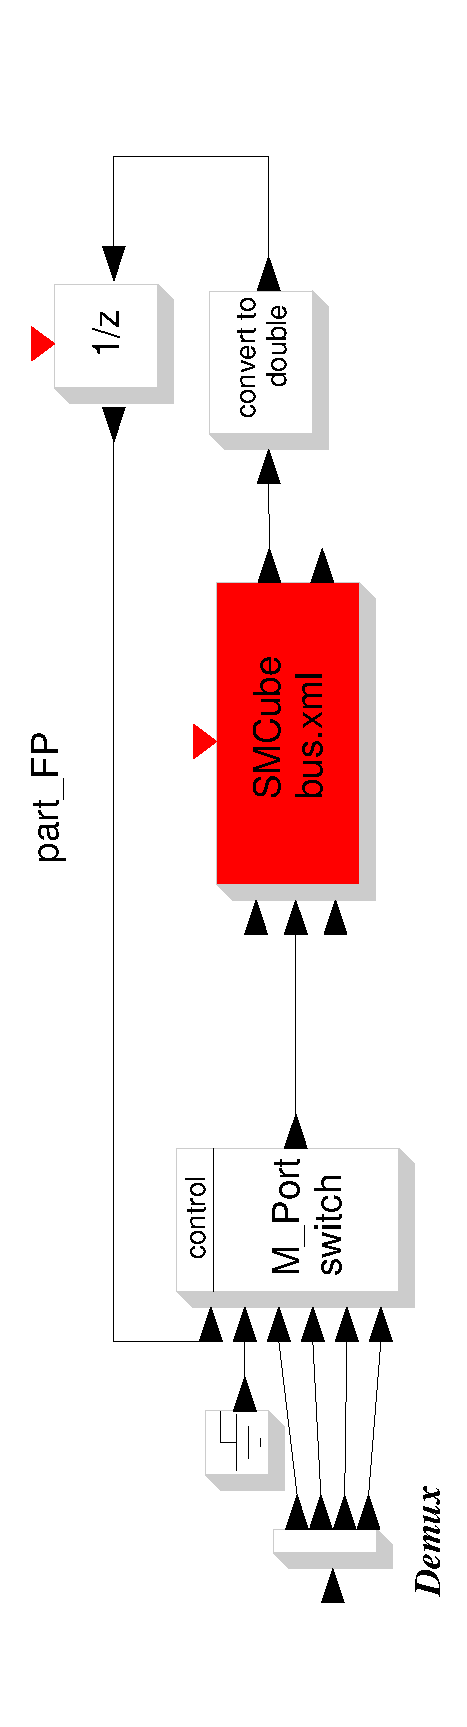
\includegraphics[angle=-90, width=1.2\textwidth]{smcube_block_ex.eps}}%
\caption{Blocco SMCube rappresentante un bus (in rosso) all'interno di un diagramma Scicos.}
\label{Fig:smcube_scicos_ex}
\end{figure}